\begin{Exercise}[title=Cyanide]
  \begin{center}
    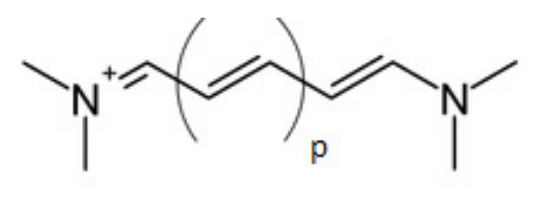
\includegraphics[width=0.3\textwidth]{cyanide.png}
  \end{center}
  Les cyanines sont une classe de molécules correspondant à des colorants organiques. Leur structure générale est présentée ci-contre. Elles sont formées d’une chaîne carbonée mettant en jeu des doubles liaisons conjuguées. Des fonctions amines sont présentes aux extrémités de cette chaîne. Divers substituants peuvent être envisagés sur les atomes d’azote. Nous examinerons le cas ici de substituants méthyle $CH^{-}_3$. Dans un modèle simple, on peut montrer que leur couleur est directement liée à leur longueur. En effet, Cette structure particulière, par des phénomènes de mésomérie, permet d’obtenir une délocalisation des électrons participant aux liaisons $\pi$. La molécule peut alors être modélisée pour ces électrons comme un fil conducteur de longueur $L$ dans lequel ils seront cantonnés.
  
\Question Etablir l’expression des longueurs d’onde possibles pour la fonction d’onde associée à un électron piégé dans un puits représenté par une boîte de longueur $L$. Déduire la quantité de mouvement de cet électron et obtenir alors les valeurs associées $E_n$ pour les énergies quantifiées accessibles à l’électron. En fonction de $h,m_e$ et $L$. 
\Question On considère le cas d’une cyanine possédant 9 atomes de carbones sur sa chaîne (p = 3 sur le schéma). La distance entre deux atomes de carbone ou un atome de carbone et un atome d’azote est $d\simeq0,14 nm$. On considèrera  que  la  délocalisation  se  fait  sur  une  longueur  correspondant  à  l’ensemble  des  liaisons impliquées, et qu’elle dépasse d’une demi-longueur de liaison à chaque extrémité.  Calculer les niveaux d’énergie correspondant en eV  jusqu’à n = 7.

\Question Combien  d’électrons  sont-ils  impliqués  dans  cette  délocalisation ?  Le  principe  d’exclusion  de  Pauli implique que l’on ne peut placer que deux électrons (de spins opposés) par niveau (on n’oubliera pas le doublet libre sur l’atome d’azote situé à droite sur le schéma, non représenté). Tracer le diagramme de remplissage dans l’état d’énergie le plus bas.
\Question Quelle est la transition pour l’excitation de plus basse énergie ? Calculer la longueur d’onde associée et expliquer la coloration de la molécule. Quelle est la couleur observée pour cette molécule ?
\Question Quelles sont les longueurs d’onde et couleurs pour des cyanines à 7 ou à 11 atomes de carbone ?
\end{Exercise}
\begin{Answer}
  \Question $\lambda = \frac{2L}{k}$. soit $E=\frac{p^2}{2m}=\frac{h^2n^2}{8mL^2}$.
  \Question $d =0.14nm $ et $ L = (N_c+1+\frac{2}{2})d$
  \Question $p=3$ on a 2 électrons par groupe $p$+ 4 sur les liaison extremes+ 2 du doublet non liant. = 12 électrons.
  \Question 2 électrons par sous couches.
  \Question $\Delta E =\frac{hc}{\lambda}=2eV $ soit $\lambda = 0.62\mu m$
\end{Answer}
